\documentclass{slides}
\usepackage{colour,epsfig,amssymb}
\textwidth=280mm
\textheight=210mm
\hoffset=-15mm
\voffset=-45mm
\parindent 0pt
\def\?{$\spadesuit$}
\def\n{\phantom{1}}
\def\D{\displaystyle}
\special{! TeXDict begin /landplus90{true}store end }

\begin{document}
\footnote[0]{\tiny\it TB 17.12.01, Peter Gl\"assel}

\mbox{\epsfig{file=Logo.ps}\hspace{5mm}
\begin{minipage}[b]{220mm}
\begin{center}
{\magenta\rule{220mm}{2mm}}\\[-10mm]
{\large\bf Low-Permeability Material in the L3 Magnet}\\
{\magenta\rule{220mm}{2mm}}\\
\vspace*{10mm}
\end{center}
\end{minipage}
}
\begin{list}
{$\bullet$}{\topsep=10pt\itemsep=0pt\parsep=5pt\labelsep=10pt\leftmargin=25pt%
  \labelwidth=15pt}

\item Cylinder-symmetric and 2-D planar calculations (POISSON):

      {\red rods along field}

      {\blue rods perpendicular to field}

\item $\mu=const$, i.e.\ linear treatment

\item Superposition principle: effects of structural elements are
additive.

\item Simulation of hollow profiles by solid rods with same {\blue
average $\mu$}

\item Bulk material $\mu=1.05$, locally higher (e.g.\ welds): $\mu =
1.7$

\end{list}

\newpage %%%%%%%%%%%%%%%%%%%%%%%%%%%%%%%%%%%%%%%%%%%%%%%%%%%%%%%%

\footnote[0]{\tiny\it TB 17.12.01, Peter Gl\"assel}

\mbox{\epsfig{file=Logo.ps}\hspace{5mm}
\begin{minipage}[b]{200mm}
\begin{center}
{\magenta\rule{200mm}{2mm}}\\[3mm]
{\bf General features of field distortion}\\
{\magenta\rule{200mm}{2mm}}\\
\vspace*{15mm}
\end{center}
\end{minipage}
}
\begin{list}
{$\bullet$}{\topsep=10pt\itemsep=0pt\parsep=5pt\labelsep=10pt\leftmargin=25pt%
  \labelwidth=15pt}

\item Maxwell's equations: $\D \frac{B_{1\perp}}{B_{2\perp}} = 1$
\hspace{10mm}
$\D \frac{B_{1\parallel}}{B_{2\parallel}} = \frac{\mu_1}{\mu_2}$

\item fieldlines are focussed into magnetic material:

      {\blue depletion} of field laterally

      locally higher field emerging from both ends of magnetic material

\end{list}

\newpage %%%%%%%%%%%%%%%%%%%%%%%%%%%%%%%%%%%%%%%%%%%%%%%%%%%%%%%%

\footnote[0]{\tiny\it TB 17.12.01, Peter Gl\"assel}

\mbox{\epsfig{file=Logo.ps,width=28mm}\hspace{20mm}
\begin{minipage}[b]{200mm}
\begin{center}
{\magenta\rule{200mm}{2mm}}\\[3mm]
{\bf Coordinate Convention}\\
{\magenta\rule{200mm}{2mm}}\\
\vspace*{3mm}
\end{center}
\end{minipage}
}

\hspace{30mm}3-D cylinder symmetry
\hspace{50mm}2-D cases

\begin{center}
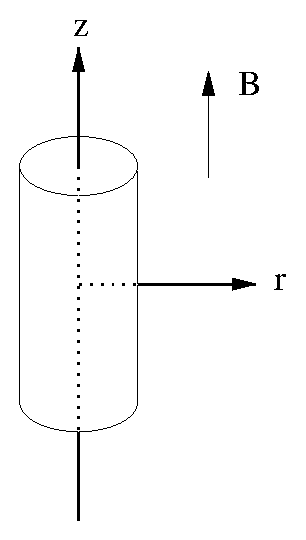
\epsfig{file=coord.eps,height=100mm}
\hspace{40mm}
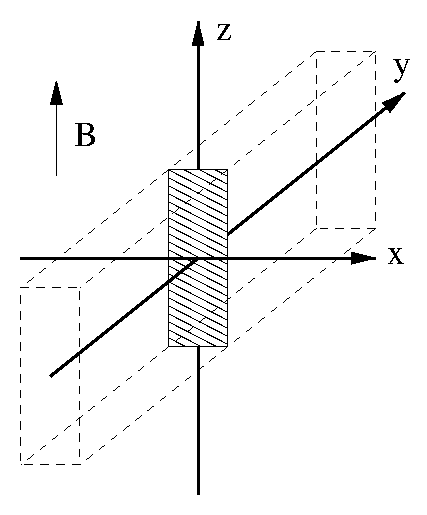
\epsfig{file=coordxy.eps,height=100mm}

\end{center}

\newpage %%%%%%%%%%%%%%%%%%%%%%%%%%%%%%%%%%%%%%%%%%%%%%%%%%%%%%%%

\footnote[0]{\tiny\it TB 17.12.01, Peter Gl\"assel}

\mbox{\epsfig{file=Logo.ps,width=28mm}\hspace{20mm}
\begin{minipage}[b]{200mm}
\begin{center}
{\magenta\rule{200mm}{2mm}}\\[3mm]
{\bf Small object}\\
{\magenta\rule{200mm}{2mm}}\\
\vspace*{3mm}
\end{center}
\end{minipage}
}
\begin{center}
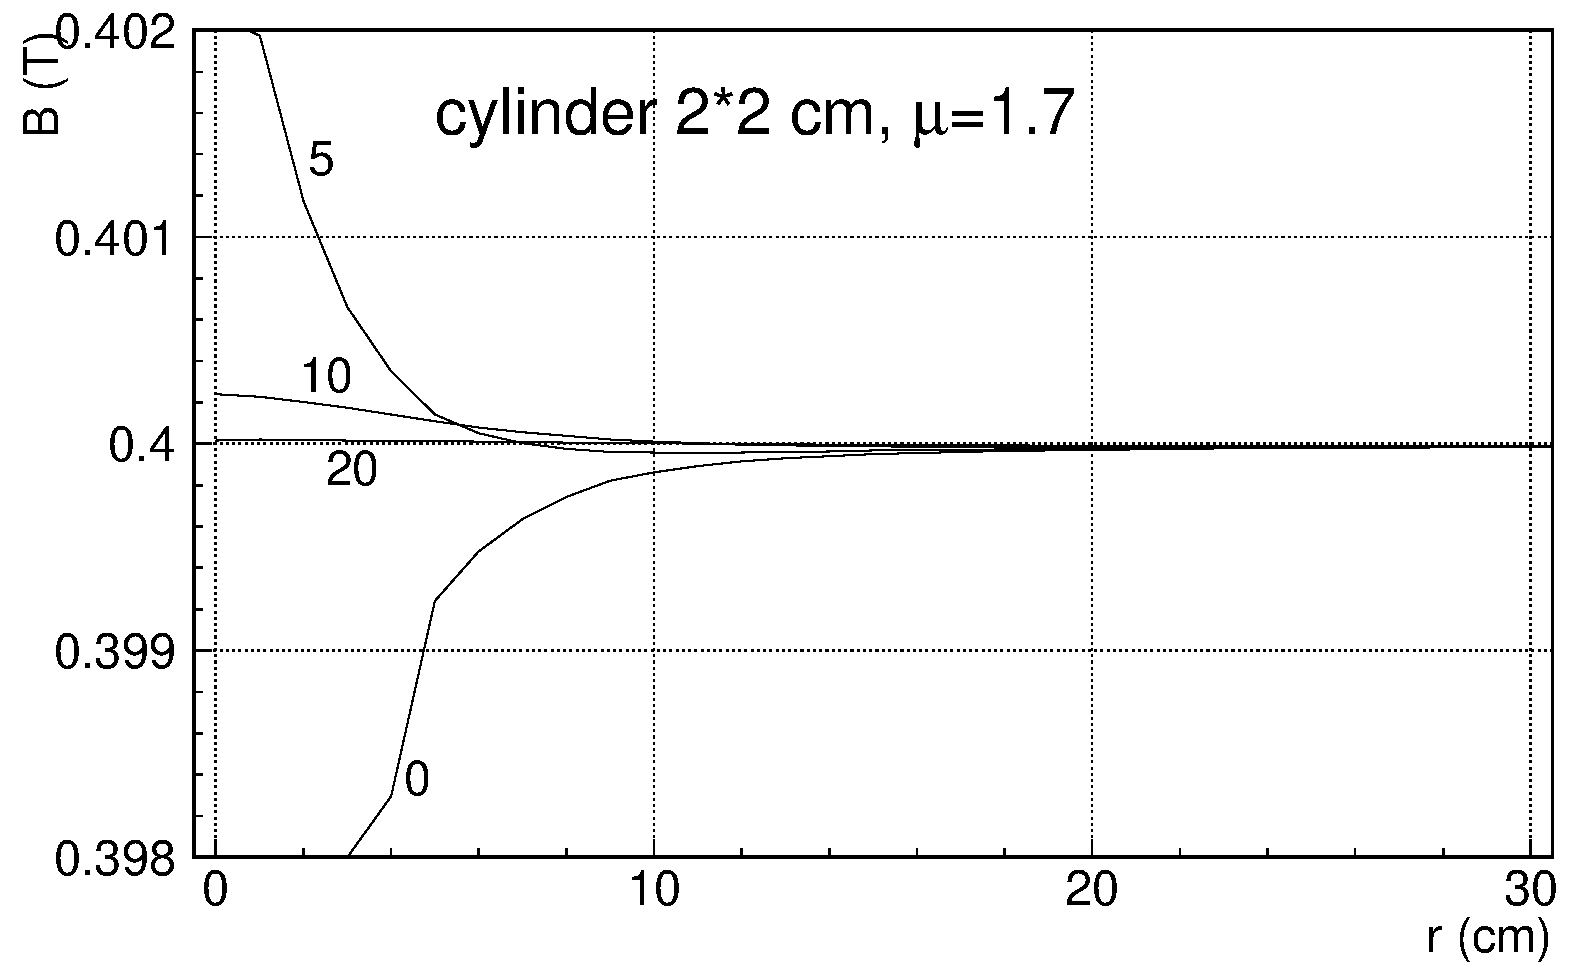
\epsfig{file=l3-2.2c.eps,height=130mm}\\
$B_z$ vs $r$ at $z=0,5,10,20$ cm from center of object
\end{center}

\newpage %%%%%%%%%%%%%%%%%%%%%%%%%%%%%%%%%%%%%%%%%%%%%%%%%%%%%%%%

\footnote[0]{\tiny\it TB 17.12.01, Peter Gl\"assel}

\mbox{\epsfig{file=Logo.ps,width=28mm}\hspace{20mm}
\begin{minipage}[b]{200mm}
\begin{center}
{\magenta\rule{200mm}{2mm}}\\[3mm]
{\bf $\mathbf{200\times 175\times 4}$ mm Space Frame Beams} \\
{\magenta\rule{200mm}{2mm}}\\
\vspace*{3mm}
\end{center}
\end{minipage}
}

%\vspace*{-10mm}
\begin{center}
%{\blue average $\langle\mu\rangle = 1.004$}\\[3mm]
\epsfig{file=l3-10c.eps,height=130mm}\\
$B_z$ vs $r$\quad end of beam at $z=0$,  $z>0$ beyond end
\end{center}

\newpage %%%%%%%%%%%%%%%%%%%%%%%%%%%%%%%%%%%%%%%%%%%%%%%%%%%%%%%%

\footnote[0]{\tiny\it TB 17.12.01, Peter Gl\"assel}

\mbox{\epsfig{file=Logo.ps,width=28mm}\hspace{20mm}
\begin{minipage}[b]{200mm}
\begin{center}
{\magenta\rule{200mm}{2mm}}\\[3mm]
{\bf Simulation of azimuthal rod $\mathbf{10\times 18\times 0.35}$ cm$^3$}\\
{\magenta\rule{200mm}{2mm}}\\
\vspace*{3mm}
\end{center}
\end{minipage}
}
\begin{center}
\epsfig{file=l3-18.10x.eps,height=130mm}\\
$B_z$ vs $x$,\quad $z$ in cm from center of rod
\end{center}

\newpage %%%%%%%%%%%%%%%%%%%%%%%%%%%%%%%%%%%%%%%%%%%%%%%%%%%%%%%%

\footnote[0]{\tiny\it TB 17.12.01, Peter Gl\"assel}

\mbox{\epsfig{file=Logo.ps,width=28mm}\hspace{20mm}
\begin{minipage}[b]{200mm}
\begin{center}
{\magenta\rule{200mm}{2mm}}\\[3mm]
{\bf Weld with $\mu=1.7$, 1 cm diameter, 20 cm long}\\
{\magenta\rule{200mm}{2mm}}\\
\vspace*{3mm}
\end{center}
\end{minipage}
}
\begin{center}
\epsfig{file=l3-20.1c.eps,height=130mm}\\
$B_z$ vs $r$,\quad $z$ in cm from center
\end{center}

\newpage %%%%%%%%%%%%%%%%%%%%%%%%%%%%%%%%%%%%%%%%%%%%%%%%%%%%%%%%

\footnote[0]{\tiny\it TB 17.12.01, Peter Gl\"assel}

\mbox{\epsfig{file=Logo.ps}\hspace{5mm}
\begin{minipage}[b]{220mm}
\begin{center}
{\magenta\rule{220mm}{2mm}}\\[-10mm]
{\large\bf Low-Permeability Material in the L3 Magnet}\\
{\magenta\rule{220mm}{2mm}}\\
\vspace*{10mm}
\end{center}
\end{minipage}
}

\begin{center}
{\large\bf Conclusions}
\end{center}

\begin{list}
{$\bullet$}{\topsep=10pt\itemsep=0pt\parsep=5pt\labelsep=10pt\leftmargin=25pt%
  \labelwidth=15pt}

\item Effect of $\mu = 1.05$ bulk material on average field: 
$\Delta B/B < 3\cdot 10^{-5}$\\
{\blue $\Rightarrow$ completely negligible}

\item Near the space frame structure: $\Delta B/B < 
10^{-3}$ for distance $d>5$ cm\\ {\blue $\Rightarrow$ acceptable}

\item Welds with $\mu = 1.7$ are unproblematic if cross sections are
small 

\item Effect of $\mu = 1.10$ beams connecting the yokes is negligible 
 
\item TPC rail ends may cause disturbance if they are too short


\end{list}
\vfill

\end{document}
